\documentclass[a4paper,10pt]{article}

\usepackage[margin=3cm]{geometry}
\usepackage{cmap}
\usepackage[T2A]{fontenc}
\usepackage[utf8]{inputenc}
\usepackage[english, russian]{babel}
\usepackage{hyperref, array, xcolor, listings, amsmath, ragged2e, forest}
\usepackage{amsmath}
\usepackage{listings}
\usepackage{graphicx}
\graphicspath{{./pictures/}}

\title{Конспекты по проге 1 семестр}
\date{}

\begin{document}
	\maketitle
	\tableofcontents
	\newpage
	
	\section{Введение}
	\subsection{Алгоритм}
	\paragraph{Определение}
		Алгоритм ― это формально описанная вычислительная процедура, получающая исходные данные (input), называемые также входом алгоритма или его аргументом, и выдающая результат вычисления на выход (output).
		Алгоритм определяет функцию (отображение):
		\begin{equation}
			F \colon X \to Y
		\end{equation}
		$X$ - входные данные, $Y$ - выходные
	\paragraph{Примеры}
	\begin{center}
	Вычисление числа Фибоначчи
	\end{center}
	\begin{lstlisting}
		int fib(int n) {
			int x = 1;
			int y = 0;
			
			for (int i = 0; i < n; i++) {
				x += y;
				y = x - y;
			}
			return y;
		}
	\end{lstlisting}
	Или же через перемножение матриц за $O(log(n))$
	\[
	\begin{pmatrix}
		F_{0} & F_{1}
	\end{pmatrix}
	\begin{pmatrix}
		0 & 1 \\
		1 & 1
	\end{pmatrix} ^ {\!\!n}
	=
	\begin{pmatrix}
		F_{n} & F_{n+1}
	\end{pmatrix}
	\]

	\begin{center}
		Проверка числа на простоту
	\end{center}
	Перебор до $\sqrt{n}$ \\
	Решето Эратосфена
	
	\begin{center}
		Быстрое возведение в степень
	\end{center}
	\begin{lstlisting}
		int power (int a, int n) {
			if (n == 0) return 1;
			if (n % 2 == 0) {
				int b = power (a, n/2);
				return b*b;
			} else {
				return power (a, n - 1)*a;
			}
		}
	\end{lstlisting}
	\newpage
	\subsection{Асимптотики}
	$f$ ограничена сверху функцией $g$ асимптотически
	\[
		f(x) \in O(g(x)) \Leftrightarrow \exists (C>0)  (\forall x) \colon \| f(x) \| \leq C \| g(x) \|
	\]
	$f$ ограничена снизу функцией $g$ асимптотически
	\[
		f(x) \in \Omega(g(x)) \Leftrightarrow \exists (C>0)  (\forall x) \colon \| f(x) \| \geq C \| g(x) \|
	\]
	$f$ ограничена сверху и снизу функцией $g$ асимптотически
	\[
		f(x) \in \Theta(g(x)) \Leftrightarrow \exists (C > 0),(C' > 0) (\forall x) \colon C \|g(x)\| \leq \|f(x)\| \leq C' \|g(x)\|
	\]
	$g$ доминирует над $f$ асимптотически
	\[
		f(x) \in o(g(x)) \Leftrightarrow \forall(C > 0) (\forall x) \colon \| f(x) \| < C \| g(x) \|
	\]
	$f$ доминирует над $g$ асимптотически
	\[
		f(x) \in \omega(g(x)) \Leftrightarrow \forall(C > 0) (\forall x) \colon \| f(x) \| > C \| g(x) \|
	\]
	$f$  эквивалентна $g$ асимптотически при $n \rightarrow n_0$
	\[
		f(n) \sim g(n) \Leftrightarrow \lim_{n \to n_0} \frac{f(n)}{g(n)} = 1
	\]
	
	\begin{center}
		Примеры \\
		$O(1) = O(2)$ \\
		$O(f(n))O(g(n)) = O(f(n)g(n))$ \\
		$f(n) \subset g(n) \Rightarrow O(f(n) + g(n)) = O(g(n))$
	\end{center}
	
	\subsection{Структура данных, абстрактный тип данных (интерфейс)}
	\paragraph{Определение} Структура данных - программная единица, позволяющая хранить и обрабатывать данные. Для взаимодействия предоставляет интерфейс.
	\begin{center}
		Примеры \\
		int a[n]; \\
		std::pair<int, int> \\
	\end{center}
	Абстрактный тип данных (АТД) - тип данных, который скрывает внутреннюю реализацию, но предоставляет весь интерфейс для работы с данными, а также возможность создавать элементы этого типа. Абстрактный тип данных реализуется с помощью структуры данных.
	\begin{center}
		Пример \\
		Стек, реализованный через массив \\
		Стек - АТД, массив - структуры данных
	\end{center}
	\newpage
	\subsection{Массив}
	\paragraph{Определение} Массив - структура данных, хранящая набор значений (элементов), которые идентифицируются по индексу или набору индексов. \\
	Динамический массив - массив, размер которого может изменяться во время выполнения программы. \\
	
	Линейный поиск - поиск по массиву за $O(n)$ \\
	В отсортированном массиве поиск возможен за $O(log(n))$ с помощью бинарного поиска \\
	\begin{lstlisting}
		int binarySearch(const int *a, int n, int item) {
    			int leftPtr = -1, rightPtr = n;

			 while (rightPtr - 1 > leftPtr) {
				int middlePtr = (leftPtr + rightPtr)/2;
				if (item > a[middlePtr]) {
					leftPtr = middlePtr;
				} else if (item < a[middlePtr]) {
					rightPtr = middlePtr;
				} else {
					return middlePtr;
				}
			}
			return rightPtr;
		}
	\end{lstlisting}
	\newpage
	\section{Базовые структуры данных}
	\subsection{Динамический массив}
	$+\colon$ random access operator \\
	$-\colon$ нельзя удалить/вставить в середину за $O(1)$
	\subsection{Односвязный и двусвязный список}
	$+\colon$ удаление и вставка в любое место \\
	$-\colon$ поиск/последовательный доступ дорог \\
	Односвязный список имеет ссылку только на следующий узел. \\
	Двусвязный список имеет ссылку на следующий и предыдущий узлы. \\
	\begin{center}
		Операции со списками: \\
		\item Поиск элемента ($O(n)$)
		\item Вставка - смена указателей ($O(1)$)
		\item Удаление - смена указателей ($O(1)$)
		\item Объединение (при условии, что храним указатель на последний элемент) - смена указателей ($O(1)$)
	\end{center}
	\subsection{Стек}
		Сертификат - Last In First Out \\
	\begin{center}
		Операции: \\
		\item Добавление в конец ($O(1)$)
		\item Удаление с конца ($O(1)$)
	\end{center}
	\begin{center}
		Можно реализовать с помощью: \\
		\item Динамического массива
		\item Списка
	\end{center}
	Для хранения в массиве можно использовать указатель на последний элемент и сдвигать его в зависимости от операции. \\
	Чтобы поддерживать минимум в стеке, достаточно хранить не элемент, а пару вида: значение элемента, минимальный элемент в стеке на момент вставки нашего элемента. \\
	\subsection{Очередь}
		Сертификат - First In First Out \\
	\begin{center}
		Операции: \\
		\item Добавление в конец
		\item Удаление из начала
	\end{center}
	\begin{center}
		Можно реализовать с помощью: \\
		\item Динамического массива
		\item Списка
		\item Двух стеков
	\end{center}
	\begin{center}
		Циклическая очередь в массиве
	\end{center}
	Реализация циклической очереди в массиве основана на хранении двух указателей: на первый элемент в очереди и на последний. Тогда удаление/вставка элементов будет связана со сдвигом указателя на первый/последний элемент по формуле newPtr = (ptr + 1)\%size \\
	\begin{center}
		Хранение очереди в списке
	\end{center}
	Для реализации на односвязном списке достаточно хранить указатель на первый и последний элемент, удаление/вставка производятся сменой указателей. \\
	\begin{center}
		Представление очереди в виде двух стеков
	\end{center}
	Для реализации очереди на двух стеках достаточно вставлять элементы в один стек, а забирать из другого. В случае, если второй стек пуст, перемещать все элементы из первого во второй. \\
	\begin{center}
		Время извлечения элемента
	\end{center}
	Для операции push возьмём 3 монеты: для самого push'а, резерв на pop из первого стека и резерв на pop из второго. Тогда учётная стоимость pop'а из второго стека будет равна 0, т.к. можно использовать оставшиеся монеты. Таким образом, каждая операция за $O(1)$ \\
	\begin{center}
		Поддержка минимума в очереди
	\end{center}
	Для поддержки минимума необходимо поддерживать минимум в каждом из стеков, тогда минимум в очереди - меньший минимум стеков. \\
	\subsection{Дек}
		Список элементов, в котором можно вставлять и удалять элементы с конца и начала.
	\begin{center}
		 Операции: \\
		 \item Вставка в конец
		 \item Извлечение из конца 
		 \item Вставка в начало
		 \item Извлечение из начала
	\end{center}
	\begin{center}
		 Можно реализовать с помощью: \\
		 \item Динамический массива
		 \item Двусвязного списка
	\end{center}
	\begin{center} 
		Хранение дека в массиве
	\end{center}
	Хранение аналогично очереди, только указатели могут сдвигаться как вперёд, так и назад (newPtr = (ptr - 1)\%size)
	\begin{center}
		Хранение дека в списке
	\end{center}
	Храним аналогично очереди, но используем двусвязный список. \\
	\subsection{Двоичная куча. АТД Очередь с приоритетом}
	\begin{center}
	\begin{forest}
		for tree={
			grow=south,
			circle, draw, minimum size=3ex, inner sep=1pt,
			s sep=7mm
			}
		[0(root)
			[1
				[3]
				[4]
			]
			[2
				[5]
				[6]
			]
		]
	\end{forest}
	\end{center}
	\paragraph{Определение}
	Двоичное подвешенное дерево, которое удовлетворяет свойствам:
	\begin{center}
		\item Значение в вершине $\leq$ ($\geq$ для максимума в корне) значению в потомке
		\item На $i$-ом слое $2^i$ вершин (кроме, возможно, последнего). Глубина кучи $\log{n}$
		\item Последний слой заполняется слева направо
	\end{center}
	\begin{center}
		Удобно хранить бинарную кучу в массиве: \\
		\item $a[0]$ - корень
		\item $a[i] \rightarrow (a[2i+1], a[2i+2])$ - потомки
	\end{center}
	\paragraph{Операции}
	Вставка за $O(\log{n})$:
	\begin{center}
		\item Вставляем в свободное место
		\item Рекурсивно поднимаем элемент, если он меньше (больше) родителя (siftUp)
	\end{center}
	Удаление за $O(\log{n})$:
	\begin{center}
		\item Удаляем минимум
		\item Вставляем последний элемент в корень
		\item Рекурсивно меняем элемент с минимальным (максимальным) потомком (siftDown)
	\end{center}
	\paragraph{Очередь с приоритетом}
	- абстрактный тип данных, который поддерживает следующие операции: 
	\begin{center}
		\item push - добавить в очередь элемент с определенным приоритетом
		\item pop - удалить из очереди элемент с наивысшим приоритетом
		\item top - посмотреть элемент с наивысшим приоритетом (необязательная операция)
	\end{center}
	\subsection{Амортизационный анализ}
	\paragraph{Определение}
	- метод подсчёта времени, требуемого для выполнения последовательности операций над структурой данных. При этом время усредняется по всем выполняемым операциям, и анализируется средняя производительность операций в худшем случае.
	\paragraph{Средняя амортизационная стоимость}
	\[
		x = \frac{\sum_{i=0}^{n} t_{i}}{n}
	\]
	$t_{i}$ - время выполнения $i$-ой операции
	\paragraph{Амортизированное (учетное) время добавления элемента в динамический массив}
	Стоимость операции add(item) \\
	Для каждой операции add(item), для которой не требуется расширение массива, будем использовать три монетки: одна для самой вставки, две в резерв. Одну из резерва положим к вставленному элементу с индексом $i$, а вторую к элементу с индексом $i - \frac{n}{2}$, где $n$ - размер массива\\
	Когда массив заполнится, у каждого элемента будет одна монетка в резерве, которую мы сможем использовать для копирования в новый массив размером $2n$ \\
	\paragraph{Метод потенциалов}
	Пусть $\Phi$ - потенциал \\
	$\Phi_{0}$ - изначальное значение \\
	$\Phi_{i}$ - состояние после $i$-ой операции \\
	Тогда стоимость $i$-й операции $a_{i} = t_{i} + \Phi_{i} - \Phi_{i-1}$ \\
	Пусть $n$ - количество операций, $m$ - размер структуры данных, тогда $a = O(f(n,m))$, если: \\
	\begin{center}
		\item $\forall i \colon a_{i} = O(f(n,m))$
		\item $\forall i \colon \Phi_{i} = O(n(f(n,m)))$
	\end{center}
	Доказательство \\
	\[
		a = \frac{\sum_{i=1}^{n} t_{i}}{n} = \frac{\sum_{i = 1}^{n} a_{i} + \sum_{i = 0}^{n-1} \Phi_{i} - \sum_{i = 1}^{n} \Phi_{i}}{n} = \frac {n \cdot O(f(n,m)) + \Phi_{0} - \Phi_{n}}{n} = O(f(n,m))
	\]
	\paragraph{Метод бух. учёта}
	Пусть операция стоит некоторое число монет. \\
	Тогда для каждой операции мы можем взять монет с запасом, чтобы хватило на следующие возможные операции (пример с динамическим массивом) \\
	Если монет хватило на все операции, то наше предположение о стоимости каждой операции (то, что мы взяли с запасом) верно \\
	(Излагаю в неформальном стиле) \\
	\subsection{Персистентный стек}
	Стек, который хранит все свои состояния \\
	Операции:
	\begin{center}
		\item Вставка: $push(i,x) \rightarrow j$, где $i$ - конкретное состояние, $x$ - элемент, который нужно вставить, $j$ - новое состояние после вставки. При вставке создаётся новое состояние стека, где хранится вставленный элемент и ссылка на состяоние, в которое его вставили.
		\item Удаление: $pop(i) \rightarrow j$. При удалении $i$ - ого состояния идём с "родителю" $i$-ого состояния и подцепляем его копию к "деду" $i$-ого состояния.
	\end{center}
	В итоге имеем доступ к любой версии стека за $O(1)$ времени и $O(n)$ памяти. \\
	Можно реализовать с помощью:
	\begin{center}
		\item Массива
		\item Списка
	\end{center}
	\section{Сортировки и порядковые статистики}
	\subsection{Задача сортировки, устойчивость, локальность}
	Coming soon
	\subsection{Квадратичные сортировки}
	Coming soon
	\subsection{Сортировка слиянием}
	Coming soon
	\subsection{Сортировка с помощью кучи}
	Coming soon	
	\subsection{Слияние отсортированных массивов с помощью кучи}
	Coming soon	
	\subsection{Нижняя оценка времени работы для сортировок сравнением}
	Coming soon
	\subsection{Быстрая сортировка}
	\paragraph{Принцип}
	Есть массив $a[0...n-1]$ и некоторый подмассив $a[l..r]$
	\begin{center}
		\item Разделим $a[l...r]$ на две части по опорному элементу $q$: $a[l...q]$ и $a[q+1...r]$ так что каждый элемент $a[l...q]$ меньше или равен $a[q]$, который не превышает любой элемент подмассива $a[q+1...r]$
		\item Подмассивы $a[l...q]$ и $a[q+q...r]$ сортируются с помощью рекурсивного вызова быстрой сортировки
	\end{center}
	\paragraph{Схема Ломуто}
	\begin{center}
		\item Выбираем $q = a[r]$
		\begin{lstlisting}
			q = a[r];
			i = l;
			for (int j = l; j < r - 1, j++) {
				if (a[j] < q) {
					swap(a[i], a[j]);
					i++;
				}
			}
			swap(a[i], a[r];
		\end{lstlisting}
	\end{center}
	\newpage
	\paragraph{Схема Хоара}
	\begin{center}
		\begin{lstlisting}
			q = A[(r + l)/2];
			i = l;
			j = r;
			while (i <= j) {
				while (a[i] < q) {
					i++;
				}
				
				while (a[j] > q) {
					j--;
				}
				if (i >= j) {
					break;
				}
				swap(a[i], a[j]);
				i++;
				j--;
			}
		\end{lstlisting}
	\end{center}
	\paragraph{Свойства}
	\begin{itemize}
		\item Локальная
		\item Недетерминированная
		\item Неустойчивая
	\end{itemize}
	\paragraph{Асимптотика}
	Дерево рекурсий
	\begin{center}
	\begin{forest}
		for tree={
			grow=south,
			circle, draw, minimum size=3ex, inner sep=1pt,
			s sep=7mm
			}
		[n
			[n/2
				[...
					[1]
				]
				[...
					[1]
				]
			]
			[n/2
				[...
					[1]
				]
				[...
					[1]
				]
			]
		]
	\end{forest}
	\end{center}
	\[
		T(n) = 2T(\frac{n}{2}) + O(n)
	\]
	Худший случай: $T(n) = T(n-1) + \Theta(n)$ (закинули один элемент от partitional) \\
	\[ 
		T(n) = \sum_{k = 1}^{n} \Theta(k) = \Theta(\sum_{k=1}^{n} k) = \Theta(n^2) 
	\]
	\newpage
	\paragraph{Среднее время работы}
	$O(n\log{n})$
	\paragraph{Доказательство}
	Пусть $X$ - суммарное количество операций сравнения с опорным элементом. Рассмотрим массив
	$[z_{0}...z_{n}]$, пусть $z_{ij} = [z_{i}...z_{j}]$ \\
	Опорный элемент дальше не участвует в сравнении $\Rightarrow$ сравнение каждой пары $\leq$ 1 раза \\
	\[
	X = \sum_{i=1}^{n-1} \sum_{j=i+1}^{n} X_{ij}
	\] 
	где $X_{ij} = 1$, если произошло сравнение $z_{i}$ и $z_{j}$, иначе 0 \\
	Применим мат. ожидание к каждой части
	\[ 
	E[X] = E[\sum_{i=1}^{n-1} \sum_{j=i+1}^{n} X_{ij}] = \sum_{i=1}^{n-1} \sum_{j=i+1}^{n} E[X_{ij}] = \sum_{i=1}^{n-1} \sum_{j=i+1}^{n} Pr(z_{i}, z_{j})
	\]		
	где $Pr(z_{i}, z_{j})$ - вероятность того, что $z_{i}$ сравнивается с $z_{j}$ \\
	Пусть все элементы различны \\
	$x$ - опорный $\Rightarrow (\forall z_{i}, z_{j} \colon z_{i} < x < z_{j} \Rightarrow$ $z_{i}$ и $z_{j}$ не будут сравниваться)  \\
	Если $z_{i}$ - опорный, то он сравнивается с каждым элементом $z_{ij}$ кроме себя \\
	Значит $z_{i}$ и $z_{j}$ будут сравниваться, когда первым в $z_{ij}$ будет выбран один из них \\
	$X_{ij} = 1 \Leftrightarrow z_{i}$ - опорный или $z_{j}$ - опорный
	\[ 
	Pr(z_{i}, z_{j}) = Pr(z_{i}) + Pr(z_{j}) = \frac{1}{j-i+1} + \frac{1}{j-i+1} = \frac{2}{j-i+1}
	\]
	где $Pr(z_{i})$ - вероятность того, что первым элементом был $z_{i}$, а $Pr(z_{j})$ - вероятность того, что первым был $z_{j}$, тогда
	\[
	E[X] =  \sum_{i=1}^{n-1} \sum_{j=i+1}^{n} \frac{2}{j-i+1}
	\]
	Пусть $k = j - i$, тогда
	\[
	E[X] =  \sum_{i=1}^{n-1} \sum_{k=1}^{n-i} \frac{2}{k+1} = \sum_{i=1}^{n-1} \sum_{k=1}^{n-i} \frac{2}{k} = \sum_{i=1}^{n-1} O(\log{n}) = O(n\log{n})
	\]
	\paragraph{Улучшения быстрой сортировки}
	\begin{itemize}
		\item Выбор медианы из первого, среднего и последнего элементов и отсечение рекурсии меньших подмассивов (с помощью сортировок вставками)
		\item Разделение на три части (применяют, если много одинаковых элементов)
	\end{itemize}
	\subsection{$k$ порядковая статистика}
	В чём суть: пусть дан массив A длиной N и пусть дано число K. Задача в том, чтобы найти в этом массиве K-ое по величине число, т.е. K-ую порядковую статистику
	\paragraph{Алгоритм}
	Пусть опорный элемент имеет индекс m \\
	Если $k == m$ $\Rightarrow$ успех \\
	Если $k < m \Rightarrow$ ищем k-ую статистику в левой части \\
	Если $k > m \Rightarrow$ ищем (k - m - 1)-ую статистику в правой части \\
	\paragraph{Асимптотика}
	Функция partition при поиске в массиве размера $n$ делает не более $n-1$ сравнений \\
	Проведём оценку сверху, будем считать, что каждый раз выбирается большая половина \\
	\[
		T(n) \leq \frac{1}/{n} \sum_{k=1}^{n} (T(max(k-1; n - k) + n - 1) = n - 1 + \frac{1}/{n} \sum_{k=1}^{n} (T(max(k-1; n - k)) = n - 1 + \frac{2}{n}\sum_{k = [n/2]}^{n-1} T(k)
	\]
	Пусть каждый раз массив делится в определенном соотношении, т.е. $\exists c T(k) \leq ck \forall k < n$
	Тогда верно:
	\[
		T(n) = n - 1 + \frac{2}/{n}\sum_{k = [n/2]}^{n-1} ck
	\]
	Здесь короче оценка с neerc, её надо разжевать и вставить сюда
	\subsection{Сортировка подсчётом}
	Пусть у нас n целых чисел в диапазоне от $0$ до $k$ \\
	Обычно применяют, если $n$ много больше $k$ \\
	\paragraph{Алгоритм}
	Заводим массив $A[k]$ \\
	Проходим по нашему изначальному массиву и инкрементируем $A[i]$, если встретили $i$ - ое число \\
	\\ В случае целых чисел просто будем сдвигать число при записи в массив, и сдвигать обратно при доступе к элементу \\
	Также можно сортироввть по ключам сложные объекты \\
	Предварительно подсчитывает количества элементов с различными ключами и разделяем результирующий массив на соответствующие блоки (длины которых как раз и равны значениям вспомогательного массива, который мы получили \\
	Затем при повторном проходе исходного массива каждый элемент копируется в специальнго отведенный его ключу блок \\
	\paragraph{Асимптотика}
	$O(n+k)$
	\subsection{Блочная сортировка}
	\paragraph{Суть сортировки}
	Блочная сортирвка применяется при равномерном распределении входных данных \\
	Т.е. мы разбиваем вхдные данные на $n$ блоков. Внутри блока же сортируем удобным образом (либо той же блочной сортировкой). Сортировка работает только в том случае, если разбиение на блоки производится таким образом, чтобы элементы каждого следующего блока были больше предыдущего
	\paragraph{Где же применяем?}
	Эту сортировку стоит применять в случае, если данные распределены равномерно, т.е. велика вероятность того, что числа редко повторяются (например, последовательность случайных чисел) \\
	\subsection{Поразрядная сортировка}
	\paragraph{Общий смысл}
	Сначала сравниваем крайний разряд, группируем элементы по значению разряда \\
	Потом сравниваем числа по следующему разряду (сравниваем внутри группы) \\
	Перед сортировкой необходимо привести все данные к единому количеству "разрядов"
	\paragraph{MSD}
	Сравниваем, начиная со старшего разряда \\
	Добавляем "пустые" элементы (когда приводим к одинаковому количеству разрядов) в конец \\
	Подходит для строк \\
	\paragraph{LSD}
	Сравниваем, начиная с младшего разряда \\
	Добавляем "пустые" элементы (когда приводим к одинаковому количеству разрядов) в начало \\
	Подходит для чисел \\
	Но необходима устойчивая сортировка каждого разряда \\
	\paragraph{Пример}
	\[
		\begin{pmatrix}
			32[9] \\
			45[6] \\
			43[7] \\
		\end{pmatrix}
		\rightarrow
		\begin{pmatrix}
			32[9] \\
			43[7] \\
			45[6] \\
		\end{pmatrix}
		\rightarrow
		\begin{pmatrix}
			32[9] \\
			43[7] \\
			45[6] \\
		\end{pmatrix}
		\rightarrow
		\begin{pmatrix}
			3[2]9 \\
			4[3]7 \\
			4[5]6 \\
		\end{pmatrix}
		\rightarrow
		\begin{pmatrix}
			[3]29 \\
			[4]37 \\
			[4]56 \\
		\end{pmatrix}
	\]	
	\paragraph{Асимптотика LSD}
	Пусть $m$ - количество разрядом \\
	$n$ - количество чисел \\
	$k$ - количество значений каждого разряда (10 для чисел) \\
	$T(n)$ - время работы устойчивой сортировки \\
	Тогда сложность $O(m(n+k))$, если устойчивая сортировка имеет сложность $O(n+k)$ (сортировка подсчётом, например)
	\paragraph{MSD для строк}
	По первому символу разделяем строки в кучи \\
	Каждую кучу делим аналогично \\
	Когда куча достигла размера 1 - элемент на месте
	\paragraph{Асимптотика MSD}
	Пусть значения разрядов меньше $b$, а количество разрядок - $k$ \\
	Если "делим хорошо" (разбиваем на разные кучки), асимптотика $\Omega(n\log_{b}n)$ \\
	Если "делим плохо" (например, возможна ситуация строк BBBBA и BBBBC), асимптотика $O(nk)$ \\
	\subsection{Бинарная быстрая сортировка}
	Аналог MSD сортировки для строк, но алфавит состоит только из 0 и 1 
	\subsection{Мастер-теорема}
	\paragraph{О чём?} Мастер теорема позволяет найти асимптотическое решение рекуррентных соотношений, которые могут возникнуть в анализе асимптотики многих алгоритмов.
	\paragraph{Формулировка} Пусть  $a \geq 1$ и $b > 1$ - константы, $f(n)$ - функция, $T(n)$ определено на множестве неотрицательных целых чисел как: 
	\[
		T(n) = a*T(\frac{n}{b}) + f(n)
	\], где $n$ - размер задачи \\
	$a$ - количество подзадач в рекурсии \\
	$n/b$ - размер каждой подзадачи \\
	$f(n)$ - оценка сложности работы вне рекурсии \\
	Пример для merge-sort 
	\[	
		T(n) = 2T(\frac{n}{2}) + f(n)
	\]	
	где $f(n)$ - затраты на слияние $(n)$\\
	
	Зачем это нужно? В зависимости от нашей функции $f(n)$:
	\paragraph{$f(n) = O(n^{c}), c < \log_{b} a)$} тогда получаем $T(n) = \Theta(n^{\log{b}a})$
	\paragraph{Пример}
	
	\paragraph{$f(n) = \Theta(n^{c} \log^{k} n), c = \log_{b} a$} тогда получаем $T(n) = \Theta(n^{c}log^{k+1}n)$
	\paragraph{Пример}
	
	\paragraph{$f(n) = \Omega(n^{c}), c > \log_{b}a$}
	
	
	\paragraph{Доказательство}
	Рассмотрим дерево рекурсии и частный случай $n = b^{k}$
	\begin{forest}
		for tree={
			grow=south,
			circle, draw, minimum size=3ex, inner sep=1pt,
			s sep=7mm
			}
		[$f(n)$
			[$f(\frac{n}{b})$
				[...
					[$f(\frac{n}{b^{i}})$]
				]
				[...
					[$f(\frac{n}{b^{i}})$]
				]
			]
			[$f(\frac{n}{b})$
				[...
					[$f(\frac{n}{b^{i}})$]
				]
				[...
					[$f(\frac{n}{b^{i}})$]
				]
			]
			[...
			]
		]
	\end{forest}
	где $i$ - уровень рекурсии, тогда на $i$ - ом уровне
 получим суммарное количество операций $a^{i}f(\frac{n}{b^{i}})$ \\
 	Тогда \[
 		T(n) = \sum_{i=0}^{\log_{b}n}a^{i}f(\frac{n}{b^{i}}) + O(n^{\log_{b}a}) 
 	\]
	$O(n^{\log_{b}a})$ - для последнего уровня рекурсии \\
	\textbf{Доказательство для А} \\
	\[
		T(n) = \sum_{i=0}^{\log_{b}n}a^{i}f(\frac{n}{b^{i}}) + O(n^{\log_{b}a}) \geq \sum_{i = 0}^{\log_{b}n} a^{i}(\frac{n}{b^{i}})^{\log_{b}a-\epsilon} + O(n^{\log_{b}a}
	\]
	Тогда 
	\[
		\sum_{i = 0}^{\log_{b}n} a^{i}(\frac{n}{b^{i}})^{\log_{b}a-\epsilon} = n^{\log_{b}a - \epsilon} \sum_{i = 0}^{\log_{b}n} a^{i} b^{-i\log_{b}a} b^{i\epsilon} = n^{\log_{b}a - \epsilon} \sum_{i = 0}^{\log_{b}n}
	\]
	Дописать надо


	
\section{Деревья}
\paragraph{Некоторые определения}
\begin{description}
	\item[дерево] - связный граф без циклов
	\item[корневой узел] - узел, не имеющий предков
	\item[лист] - узел, не имеющий потомков
	\item[внутренний узел] - узел, имеющий потомков
\end{description}
	\subsection{Обход дерева}
\paragraph{Обход в глубину} Для обхода в глубину удобно использовать стек, в который по очереди в зависимости от порядка обхода кладется вершина, ее левый и правый ребенок. 
\paragraph{pre-order(прямой обход)}
\begin{enumerate}
	\item  Проверяем текущий узел на NULL
	\item  Выводим значение в текущем узле
	\item  Обходим прямым обходом левое поддерево
	\item  Обходим прямым обходом правое поддерево
\end{enumerate}

\paragraph{in-order(центрированный обход)}
\begin{enumerate}
	\item  Проверяем текущий узел на NULL
	\item  Обходим центрированным обходом левое поддерево
	\item  Выводим значение в текущем узле
	\item  Обходим центрированным обходом правое поддерево
\end{enumerate}

\paragraph{post-order(обратный обход)}
\begin{enumerate}
	\item  Проверяем текущий узел на NULL
	\item  Обходим обратным обходом левое поддерево
	\item  Обходим обратным обходом правое поддерево
	\item  Выводим значение в текущем узле
\end{enumerate}

\paragraph{Обход в ширину} - значения в вершинах выводятся по уровням слева направо\\
Для осуществления такого обхода надо завести очередь и положить в нее корень дерева. Пока очередь непуста, достаем из нее элемет, выводим его значение и кладем в очередь его левого и правого ребенка.
\subsection{Двоичное дерево поиска}
У каждой вершины не более 2х потомков, любое поддерево так же является деревом поиска, все ключи в левом поддереве меньше, чем в корне, в правом поддереве - больше, чем в корне. 
\paragraph{Поиск} - по ключу возвращаем ссылку на узел с таким же ключом\\
\begin{\textbf{Алгоритм}}
	\item Если текущий узел пуст - вернуть NULL
	\item Если ключ текущего узла равен искомому - вернуть ссылку на текущий узел 
	\item Если ключ текущего меньше искомого - уйти в левое поддерево, иначе - в правое
\end{itemize}
\paragraph{Вставка} - рассматриваем случай, когда все ключи различны\\
\begin{\textbf{Алгоритм}}
	\item Если дерево пусто - заменить корень на узел с ключом равным данному, завершить работу
	\item Если ключ текущего меньше искомого - уйти в левое поддерево, иначе - в правое
\end{itemize}
\paragraph{Удаление}\\
\begin{\textbf{Алгоритм}}
	\item Если текущий узел пуст - завершить работу
	\item Если ключ текущего меньше данного - рекурсивно удалить ключ из левого поддерева, иначе - из правого
	\item Если ключ текущего узла равен искомому - рассмотреть случаи 
	\begin{enumerate}
		\item текущий узел - лист - удалили и не паримся
		\item у текущего узла один ребенок - поставили ребенка вместо текущего узла, текущий удалили
		\item у текущего узла два ребенка - возьмем m самый левый узел правого поддерева, удалим его из правого поддерева, поставим вместо текущего ключа ключ m
	\end{enumerate}
\end{itemize}
\subsection{Декартово дерево}
Курево(куча + дерево) - бинарное дерево, в узлах которого хранятся пары (ключ, приоритет). По ключам курево является двоичным деревом поиска, а по приоритетам - кучей.
\paragraph{split} - по дереву Т и ключу к split возвращает 2 дерева Т1 и Т2. В Т1 все ключи меньше к, в Т2 все ключи больше или равны к.\\
\textbf{Псевдокод}\\
\begin{center}
		\begin{lstlisting}
			<Treap*, Treap*> split(Treap* t, Key k){
				if(t == NULL) return <NULL, NULL>;
				if(t->key > k){
					<t1, t2> = split(t->left, k);
					t->left = t2;
					return <t1, t>;
				}else{
					<t1, t2> = split(t->right, k);
					t->right = t1;
					return <t, t2>;
				}
			}
		\end{lstlisting}
	\end{center}
Время работы алгоритма - О(h), где h - высота дерева, т.к. split рекурсивно проходит по вершинам в глубину дерева и на каждом шаге работает О(1)
\paragraph{merge} - по двум куревам Т1 и Т2, любой ключ в Т1 меньше любого ключа в Т2, merge строит курево Т, в котором есть все ключи из первого и второго дерева.\\
\textbf{Псевдокод}\\
\begin{center}
		\begin{lstlisting}
			Treap* merge(Treap* t1, Treap* t2){
				if(t1 == NULL) return t2;
				if(t2 == NULL) return t1;
				if(t1->priority > t2->priority){
					t1->right = merge(t1->right, t2);
					return t1;
				}else{
					t2->left = merge(t1, t2->left);
					return t2;
				}
			}
		\end{lstlisting}
	\end{center}
Время работы алгоритма - О(h), где h - высота дерева, т.к. split рекурсивно проходит по вершинам в глубину дерева и на каждом шаге работает О(1)
\paragraph{Вставка узла}\\
split по ключу вставляемого узла\\
merge первого курева из возвращенной пары и вставляемого узла\\
merge этой штуки  с оставшимся куревом
\paragraph{Удаление по ключу}\\
split по ключу удаляемого узла\\
из второго курева из возвращенной пары удалим самого левого ребенка\\
merge этой штуки  с оставшимся куревом
\paragraph{Построение} - наивно - просто добавлять по порядку, каждая вставка за  О(log n), значит общая сложность  О(n log n)\\

\textbf{Алгоритм за O(n)} - если пары отсортированны по ключу по возрастанию\\
Будем строить дерево слева направо, то есть начиная с (x1,y1) по (xn,yn), при этом помнить последний добавленный элемент (xk,yk). Он будет самым правым, так как у него будет максимальный ключ, а по ключам декартово дерево представляет собой двоичное дерево поиска. При добавлении (xk+1,yk+1), пытаемся сделать его правым сыном (xk,yk), это следует сделать если yk>yk+1, иначе делаем шаг к предку последнего элемента и смотрим его значение y. Поднимаемся до тех пор, пока приоритет в рассматриваемом элементе меньше приоритета в добавляемом, после чего делаем (xk+1,yk+1) его правым сыном, а предыдущего правого сына делаем левым сыном (xk+1,yk+1).\\
Заметим, что каждую вершину мы посетим максимум дважды: при непосредственном добавлении и, поднимаясь вверх (ведь после этого вершина будет лежать в чьём-то левом поддереве, а мы поднимаемся только по правому). Из этого следует, что построение происходит за O(n).
\paragraph{Теорема про случайные приоритеты} по сути про то, что глубина О(n log n)\\
coming soon...\\

\subsection{АВЛ - дерево}

	\paragraph{Основное свойство} - сбалансированность \\
	Для каждой вершины $|h(l) - h(r)| \leq 1$, где $h(l)$ - глубина левого поддерева, $h(r)$ - глубина правого поддерева \\
	
	\paragraph{Высота} $O(\log N)$ \\
	\textbf{Доказательство} - по индукции докажем, что минимальное число вершин в AVL-дереве высоты $h$: $m_{h} = F_{h+2} - 1$, где $F_{h}$ - $h$-ое число Фибоначчи. \\
	$m_{h+2}$ = $m_{h+1} + m_{h} + 1$, т.к. разница между высотой детей не больше 1. \\
	Далее доказательство по индукции.\\
	$F_{h} = \Omega(\phi^{h})$, где $\phi$ - константа. \\
	Получаем $n \geq \phi^{h} \Leftrightarrow \log_{\phi} n \geq h$ \\
	
	\textbf{Как балансировать дерево?} - очень просто \\
	Поворот производим, если разница высот равна 2. \\
	Существует два основных типа поворота - правый и левый, но не всегда мы можем сразу выполнить поворот. \\
	Мы можем сделать левый поворот, если высота правого ребёнка больше левого и \textbf{высота правого ребёнка правого ребёнка (т.е. самого правого внука изначальной вершины) больше или равна высоте левого ребёнка правого ребёнка} \\
	Правый поворот при аналогичных условиях, т.е. высота левого ребёнка больше правого и \textbf{высота левого рёбёнка левого рёбнка (т.е. самого левого внука изначальной вершины) больше или равна высоте правого ребёнка левого ребёнка} \\
	\textbf{Как выполняется поворот?} - разберём на примере левого поворота, для правого аналогично \\
	Мы "поднимаем" правого ребёнка наверх, при этом он неожиданно становится родителям троих детей, так у нас не принято, поэтому одного ребёнка нужно отдать другому ребёнку, отличный кандидат для этого - предыдущий левый ребёнок правого ребёнка, т.к. неожиданно у нашей рассматриваемой ноды (для которой мы осуществляли поворот) остался только один ребёнок. \\
	
	\textbf{Звучит сложно?} Тогда посмотрим картинки. \\
	
	\begin{center}
	\textbf{Выполняем левый поворот. Случай, когда правый ребёнок правого ребёнка больше.} \\
	\begin{forest}
		for tree={
			grow=south,
			circle, draw, minimum size=3ex, inner sep=1pt,
			s sep=7mm
			}
		[5
			[3
			]
			[10
				[7
				]
				[15
					[12
					]
					[20
					]
				]
			]
		]
	\end{forest} \\
	
	\textbf{Дерево переходит в следующий вид} \\
	
	\begin{forest}
		for tree={
			grow=south,
			circle, draw, minimum size=3ex, inner sep=1pt,
			s sep=7mm
			}
		[10
			[5
				[3
				]
				[7
				]
			]
			[15
				[12
				]
				[20
				]
			]
		]
	\end{forest}
	\end{center}
	
	Если же мы не можем сразу сделать поворот, но баланс нарушен, то нужно спуститься к ребёнку (правому, если у нас левый поворот, иначе левому) и сделать поворот в другую сторону уже относительно него, чтобы привести дерево в подходящий вид. \\
	\textbf{Посмотрим картинки} 
	\begin{center}
	\textbf{Выполняем левый поворот. Случай, когда левый ребёнок правого ребёнка больше, поэтому сначала делаем правый поворот для правого ребёнка} \\
	\begin{forest}
		for tree={
			grow=south,
			circle, draw, minimum size=3ex, inner sep=1pt,
			s sep=7mm
			}
		[5
			[3
			]
			[10
				[7
					[6
					]
					[8
					]
				]
				[15
				]
			]
		]
	\end{forest} \\
	\textbf{Для начала сделаем правый поворот для правого ребёнка} \\
	\begin{forest}
		for tree={
			grow=south,
			circle, draw, minimum size=3ex, inner sep=1pt,
			s sep=7mm
			}
		[5
			[3
			]
			[7
				[6
				]
				[10
					[8
					]
					[15
					]
				]
			]
		]
	\end{forest} \\
	\textbf{Теперь можем спокойно сделать левый поворот} \\
	\begin{forest}
		for tree={
			grow=south,
			circle, draw, minimum size=3ex, inner sep=1pt,
			s sep=7mm
			}
		[7
			[5
				[3
				]
				[6
				]
			]
			[10
				[8
				]
				[15
				]
			]
		]
	\end{forest} \\

	\end{center}

\subsection{Красно-черное дерево}
 двоичное дерево поиска, в котором баланс осуществляется на основе "цвета" узла дерева, который принимает только два значения: "красный" и "чёрный"\\
При этом все листья дерева являются фиктивными и не содержат данных, но относятся к дереву и являются чёрными. "Объединим" их в один NIL\\
\paragraph{Свойства}
\begin{enumerate}
	\item Каждый узел промаркирован красным или чёрным цветом
	\item Корень и конечные узлы (листья) дерева — чёрные
	\item У красного узла родительский узел — чёрный
	\item Все простые пути из любого узла x до листьев содержат одинаковое количество чёрных узлов
	\item Чёрный узел может иметь чёрного родителя
\end{enumerate}
\paragraph{Высота красночерного дерева}\\
Черная высота вершины x - число чёрных вершин на пути из x в лист.\\
\textbf{Лемма} В красно-черном дереве высотой $hb$ количество внутренних вершин не менее $2^{hb-1}-1$\\
доказывается по индукции по высоте дерева\\
\textbf{Теорема} Красно-черное дерево с n ключами имеет высоту О(log n)\\
Рассмотрим красно-чёрное дерево с высотой $h$. Так как у красной вершины чёрные дети (по свойству 3) количество красных вершин не больше $\frac{h}{2}$. Тогда чёрных вершин не меньше, чем $\frac{h}{2} - 1$\\
По лемме для дерева размера n\\
$n \leq 2^{\frac{h}{2}}-1$\\
Прологарифмировав неравенство, имеем:\\
$h \leq 2log(n+1)$\\
\paragraph{Вставка}\\
Вставка узла производится на мето NIL'а. Вставляем вершину вместо NIL с нулевыми потомками и красим в красный цвет.
\begin{Балансировка для вершины х}
	\item[]Отец - черный - все ок
	\item[]Отец - красный - нарушается свойство 3 (при этом отец точно не корень, значит есть и дедушка)\\
\begin{enumerate}
	\item Дядя - красный\\
		Перекрасим отца и дядю в черный, деда в крассный. Поддерево с вершиной х - сбалансированно. Теперь балансируем деда.\\
\begin{center}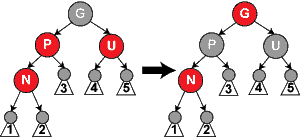
\includegraphics{rbt_in_ru.png}\end{center} 

	\item Дядя - черный\\
Пусть о - отец, д - дед, т - дядя вершины х\\
		Рассмотрим случай, когда о - левый ребенок д. Правый симметрично\\
		Если х - правый ребенок о, выпоним левый поворот: о становится левым ребенком х, х становится на место о.\\
		Теперь можем совершить правый поворот, т.е. корнем поддерева станет левый ребенок д, д станет правым ребенком нового корня. Т.к. до вставки х дерево было сбалансированно, д - черная вершина. Перекрасим д в красный, новый корень в черный. Свойства сохранятся\\
\begin{center}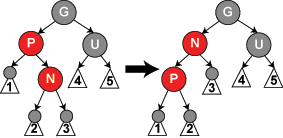
\includegraphics{rbt_in_bu.png}\end{center} 
\end{enumerate}
\end{description}
\paragraph{Удаление}(видимо тебя из этой жизни)\\
\begin{Удаление в зависимости от количества детей}
	\item Если у вершины нет ненулевых детей, то баланируем и изменяем указатель на неё у родителя на NIL
	\item Если у неё только один ненулевой ребёнок, то балансируем и делаем у родителя ссылку на него вместо этой вершины.
	\item Иначе находим наименьший элемент в правом поддереве(сначала мы переходим в правое поддерево, а после спускаемся вниз в левое до тех пор, пока у вершины есть левый ненулевой ребенок), копируем его значение в удаляемый, удаляем его рекурсивно из правого поддерева по 1му или 2му пункту.
\end{enumerate}
Заметим, что балансировать удаляемую вершину, у которой 2 ребенка не надо, т. к. в ней ничего не изменилось, кроме значения, а значит свойства могли сломаться только у наименьшего элемента в правом поддереве, который мы удалили.
А дальше - балансировка!\\
Если вершина была красной, то и балансировать даже не надо.
Если она была черной, то если ее ребенок был красным, просто перекрасим его в черный.\\
Иначе и удаляемая вершина и ее ребенок - черные.\\
Дальше рассматриваем случай, когда n - левый ребенок. Правый симметрично.
Итак, удалили вершину n, на ее месте теперь ребенок n и он черный(нзовем его х). Исходим из того, что брат х - черный.\\
Если брат х - красный, то совершим левый поворот вокруг нового родителя х, перекрасим родителя в красный, а брата в черный. Сейчас брат стал дедушкой х. Т.к. он был красный, его дети черные, его левый ребенок стал братом х, значит у х сейчас черный брат.\\
\begin{center}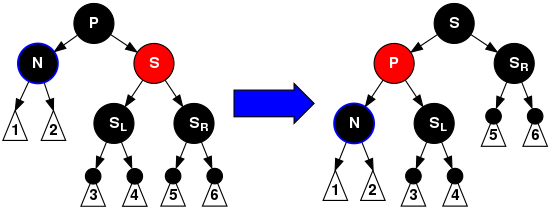
\includegraphics[scale=0.7]{rbt_del_1.png}\end{center} 
Теперь рассмотрим случаи:
\begin{enumerate}
	\item Если оба ребенка брата - черные, перекрасим брата в красный. Тогда поддерево с корнем в родителе х сбалансированно. При этом, если родитель х был красным, перекрасим его в черный и дерево окажется сбалансированным, иначе все пути, идущие через родителя х, имеют черную глубину на один меньше, чем все остальные. Тогда запустим балансировку от родителя\\
\begin{center}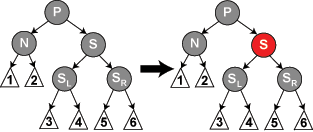
\includegraphics{rbt_del_2.png}\end{center}
	\item Если левый ребенок брата - красный, а правый - черный, то совершим правый поворот вокруг брата. Его красный ребенок станет новым отцом. Поменяем цвета нового отца и брата. у х теперь есть черный брат с черным левым и красным правым потомком. Переходим к следующему случаю.\\
\begin{center}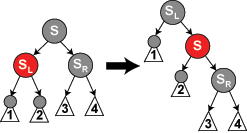
\includegraphics{rbt_del_4.png}\end{center}
	\item Левый ребенок брата - черный, а правый - красный. Совершим поворот относительно отца х влево. Поменяем цвета отца и брата местами, т.е. отец станет черным, а черная высота левого поддерева брата(нового отца) увеличится на 1, а правого уменьшится на 1. Перекрасим правого ребенка брата в черный\\
\begin{center}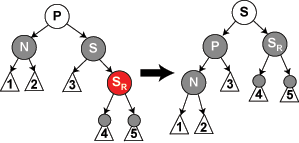
\includegraphics{rbt_del_5.png}\end{center}
\end{enumerate}
\paragraph{Оценка сложности(прямо с wiki, так что придется подкорректировать)}\\
Все рекурсивные вызовы функции хвостовые и преобразуются в циклы, так что алгоритм требует памяти O(1). В алгоритме выше, все случаи связаны по очереди, кроме случая 3, где может произойти возврат к случаю 1, который применяется к предку узла: это единственный случай когда последовательная реализация будет эффективным циклом (после одного вращения в случае 3).

Так же, хвостовая рекурсия никогда не происходит на дочерних узлах, поэтому цикл хвостовой рекурсии может двигаться только от дочерних узлов к их последовательным родителям. Произойдет не более, чем O(log n) циклических возвратов к случаю 1 (где n — общее количество узлов в дереве до удаления). Если в случае 2 произойдет вращение (единственно возможное в цикле случаев 1-3), тогда отец узла N становится красным после вращения и мы выходим из цикла. Таким образом будет произведено не более одного вращения в течение этого цикла. После выхода из цикла произойдет не более двух дополнительных поворотов. А в целом произойдет не более трех поворотов дерева.
\end{document}
